\chapter{Objective}\label{chObjective}
	In the first section the chapter introduces the purposes of the working team and motivates the choices of the objectives of the software. Then, in the second one, it presents the goals of the software and, in the third, the requirements.
 
\begin{comment}
The objective of the work is composed by the goals the software have to reach and the definition of the requirements for achieving them. These two aspects are described in the following sections.
\end{comment}

	\section{The Context}
	The work presented in the following chapters is a subset of the work of a research group, which aims to provide \mbox{ACT-R} of a visual system which is as similar as possible to the human one. 
	As this objective is very broad, this work focuses only on a particular subset of tasks.

	%As this goal is very ambitious and the author of this document has been introduced in a team with specific sub-goals only for a limited amount of time, he focused on particular tasks. Such tasks are described in the next sections.

	%The final purpose of this work is to provide \mbox{ACT-R} of a complete visual system, which is as similar as possible to the human one. 
	%This fact represents a huge challenge for the research world. 
	To reach such goal, the researchers continuously monitor the progresses in the computer vision research field in order to find useful innovative techniques to combine with consolidated solutions. 
	Such search, anyway, it is not easy. In fact, although computer vision studies are very active and find every year new algorithms able to solve different problems, often such algorithms introduce contextual information that makes them tasks specific: they are suitable to solve only the specific tasks for which they are designed. 
	For this reason, it is very difficult to find a general purpose solution which is able to make machine vision system behave like the human one.


%	Like most of research works, this project requires an unknown time to produce final and acceptable results.
	Like most of research works, this project has to deal with a certain degree of uncertainty that makes difficult to set any time constraints.
	The author of this work, however, has been inserted for a limited time interval in a team composed by three people, whose aim is to implement particular solutions in order to solve specific tasks. 
	For this reason the following parts of this document describe only the features developed during this amount of time by the author, explaining them in the context of the objectives of the team. 
	
		\subsection{The Goal of the Team}\label{goalTeam}
		The goal of the team is to create a general purpose software, which receives as input a video stream or an image and performs an object recognition process.
		\mbox{ACT-R} uses the information obtained by this tool to orientate inside a building.
% by distinguishing different categories of rooms thanks to the objects they contain.
		In particular, the software analyzes a video looking for objects and transmits all the recognized items to a model developed in \mbox{ACT-R}. The model has to distinguish different categories of rooms basing on the information about the objects they contain.

		As a starting point for such software, the team has to implement a tool for recognizing geometrical shapes in the input images. Such software has to accomplish two goals: the first one is to extract a subset of all the features in the image, in order to simplify the object recognition process; the second one is to make easier the definition of models for the modelers. This tool, which represents the main topic of this work, is described better in the next sections. 
%\end{comment}
		

%\todo{sistemare}
\begin{comment}
		The goal of the team is to create a general purpose software, which receives as input a video stream and performs an object recognition process. 
		\mbox{ACT-R} uses the information obtained by this tool in combination with its intelligence to orientate a robot inside a building and drive it through the structure. The robot has a camera mounted on it that transmits the video stream to the object recognition tool. This instrument analyzes the video looking for objects and transmits all the recognized ones to the artificial intelligent framework, that takes all the decisions necessary to drive the robot. 
	
		As a starting point for such software, the team has to implement a tool for recognizing geometrical shapes in the input images. Such software has to accomplish two goals: the first one is to extract a subset of all the features in the image, in order to simplify the object recognition process; the second one is to make easier the definition of models for the modelers. This tool, which represents the main topic of this work, is described better in the next sections. 
\end{comment}

	\section{The Goals of the Software}\label{TeamGoal}
	The software to be designed and developed is a visual module for the cognitive architecture ACT-R, whose aim is to improve ACT-R visual perception in order to make it more similar to the human one. 
	
	In order to develop a model in ACT-R, the modelers need a series of parameters on which basing their assumptions about the model itself and its performances.
	The collection of such data is accomplished thanks to experiments in which human beings take part. 
	For every experiment a specific program is created in order to measure some variables as, for example, the time needed to complete a task and the accuracy of the result.
	The parameters obtained by these experiments are then used as a reference for the development of ACT-R model.

\begin{comment}
After a model is developed in ACT-R, it needs to be validated . Model validations usu-
ally are realized with experiments in which human beings take part. For every experiment
a specific program is created in order to measure some variables as, for example, the time
needed to complete a task and the accuracy of the result. The parameters obtained by
the model are then comparemd with the ones obtained in these experiments.
\end{comment}


 
	Image~\ref{fig:RushHourHuman} shows a test case of an experiment in which the goal is to solve some levels of the game \emph{Rush Hour}. As shown, the grid contains some colored rectangles, each of which represents a car. The player must free the red one making it go out of the grid through the exit on the right. The cars can be moved only in the horizontal and vertical directions, according to their orientation. %The goal of the game is to free the red car. 
	The lower the number of moves, the better is such solution.

	\begin{figure}[!h]
	  \begin{center} 
	    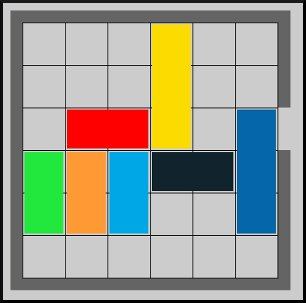
\includegraphics[scale=0.6]{images/ch_03/originale.jpg}	
	  \end{center} 
	  \caption{\textit{Example of level of Rush Hour game}}
	  \label{fig:RushHourHuman}	
  	\end{figure}
	
	In order to conduct an experiment, the modelers prepare a set of instances of the problem and every person who is going to participate to the experiment has to face a fixed number of them.
	For each instance, the ad-hoc program shows the image with the initial configuration (figure \ref{fig:RushHourHuman}) and the person has to give the solution of the game by clicking on the rectangles in the order he thinks to be correct. As the program never updates the image, the player has to imagine the solution. The software manages to interpret the direction of the shift by analyzing the movement of the eye, thanks to a module of \emph{eye tracking}. Moreover, it records the movements of the mouse, the clicks of the mouse, the time needed to give the solution and the correctness of the solution. 

	The model written in ACT-R in order to solve a particular instance of Rush Hour problem needs to receive as input the initial configuration. At the moment, such configuration is not an image, like the one shown to people during the experiment; rather it is a list of objects written in the language of the model.
	A desirable improvement of the model should be introducing an object recognition algorithm able to detect the rectangles in the image and generate the correspondent object list in ACT-R language. 
	This approach would make ACT-R visual system more similar to humans'. Moreover, it would make more scalable the process of creating instances for the experiments. 


\begin{comment}
	The models written in ACT-R that need to process images, like the one used to solve the rush hour game, at the moment skip the image processing step and start directly from a list of objects which is written directly in the input of the model. ACT-R can not accomplish this task because its visual module does not provide functions for the image processing.
	This fact represents a big limitation for the architecture and leads to a significant gap between the human cognitive system and the framework one. In addition, writing the objects in a model leads to other problems as, for example, the loss of time to write the object for every single test, the consequent delay of the work and the non-scalability of this approach.
\end{comment}
	
	%The goal of the developed software is to reduce the gap between the human and ACT-R visual systems, being a starting point for a complete and general purpose tool for the cognitive architecture to recognize objects. 
	The purposes described above represent the goals of the tool.
	To achieve them, the software analyzes the image created for the user, processes it extracting the features needed by \mbox{ACT-R} and stores the information in dedicated data structures. Then, when \mbox{ACT-R} requests them, it communicates all the stored data to the cognitive architecture using a format compatible with \mbox{ACT-R} model. 
	

\begin{comment}
	The goals of the software  are to simplify the psychologists work of defining new test cases for experiments in ACT-R and to recognize objects during the navigation of robots.

	At the moment, a psychologist, in order to insert a new test in ACT-R, has to create two interfaces, one for the user and one for ACT-R.
	The interface for the user is generally an image and can be created with any graphical editor. 
	The interface for ACT-R, instead, is much more complicated and requires the creator of the experiment to write each shape directly on the visual buffer. \todo{check correctness of this} \todo{check if the visual buffer has been introduced}
	
	The following picture shows an example of the two images used in the test.
	The one on the left is the image shown to the user while the image on the right represents the ACT-R one. 
		
	\begin{figure}[h]
	  \begin{center} 
	    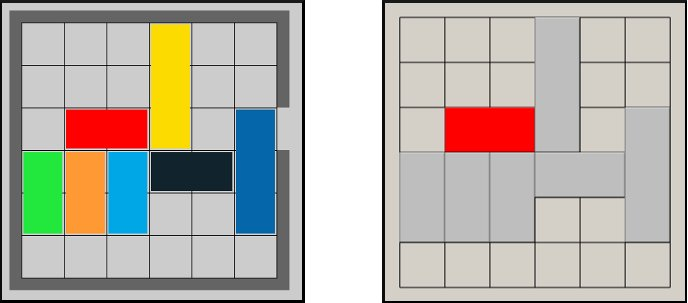
\includegraphics[scale=0.6]{images/ch_03/original_and_visicon.jpg}
	  \end{center} 
	  \caption{\textit{The two versions of the image: on the left the image for the use, on the right the image shown in ACT-R}}  
	  \label{fig:OriginalAndVisiconImages}
  	\end{figure}

	

	So, to create a test, the psychologist has to create the same image in two different formats.
	This double work causes a loss of time for the psychologist. Moreover, writing by hand all the shapes on ACT-R visual buffer is a low-level activity and can lead to stress and consequently to errors.


	The purpose of the software is to avoid to the psychologists the activity of writing on ACT-R visual buffer. To achieve this, the software analyzes the image created for the user, processes it extracting the features needed by ACT-R and communicates them to the artificial intelligence framework, which designs them automatically on its visual buffer. 
	This relieves the creators of the test of the double task described above leading to a better working experience, a less stressed work and a lower probability of errors.
	

	\todo{will i put this? or will i put it in the future developments? at the beginning it was a requirement. Will i say that the object recognition part is not developed yet?}
\end{comment}


	\section{Requirements}
	The requirements are grouped in the following sections according to the functional/non-functional classification. 
	%The simple shapes recognized are circles, triangles, squares, rectangles and ellipses.
	%Another important feature that must be introduced is the recognition of the text

		\subsection{Functional Requirements}
		The objective of the work is to design and implement a standalone software module which receives as input an image and is able to analyze it and extract some features of it.

		The input image is a color image which contains simple shapes. The shapes must not be overlapping and must have the same color hue.

		The software must recognize simple shapes, in particular:
		\begin{itemize}
	    		\item triangles;
			\item rectangles;
			\item quadrilaterals;
			\item circles.
		\end{itemize}

		For each shape, it must calculate:
		\begin{itemize}
		    	\item area;
		    	\item perimeter;
			\item dimensions;
			\item rotation;
			\item a rectangular bounding box;
			\item center;
		\end{itemize}

		Moreover, the software has to:
		\begin{itemize}
			\item recognize the color of a single pixel;
			\item recognize the color of a shape;
		    	\item calculate distances between objects;			
			\item make dimensional comparisons between objects;
			\item calculate the relative position of one object in respect with another one.
		\end{itemize}

\begin{comment}
		The shapes to be recognized are circles, triangles, rectangles and squares. 
		The color of the object is calculated averaging all the pixels of the object.
		The rotation is defined as the angle between the less sloped segment of the boundary of the object and the horizontal direction, calculated in the counterclockwise order.
		The bounding box is a rectangle whose coordinates are calculated getting the minimum and the maximum coordinates in the horizontal and vertical directions of the pixel of the image. 
		The center of a shape is the center of the bounding box.
		The distances between objects are calculated in two different ways. The first one is the distance between the centers of two shapes. The second one is the minimum distance calculated between each vertex of the bounding box of the first shape and all the vertexes of the bounding box of the second shape.
		The dimensional relation between two objects is made comparing their areas. 
		The relative position of two objects is found comparing the positions of the two top-left vertexes of each bounding box.
\end{comment}

		The software must be able to communicate with ACT-R. 
		In particular, ACT-R must signal to it which is the image to process and ask for the features to be extracted. The module must return all the information extracted by ACT-R.

		\subsection{Non-Functional Requirements}

			\subsubsection{Product Requirements}
			The software module must:
			\begin{itemize}
				\item be multi-purpose;
				\item be portable;
			    	\item work in background;			
				\item communicate with \mbox{ACT-R}.			
			\end{itemize}
			

				\paragraph{Multi-Purpose}

				The software should be easily adapted to work with all the experiments that will be put in place in the future. Moreover, there should be the possibility to adapt the software in order to use it as a shape recognition tool in the navigation with robots. For this topic, see~\ref{goalTeam}. 				
			
				\paragraph{Portability} 
				The software has to work on several operating systems.
			
				\paragraph{Communication with ACT-R} 			
				The software must transmit the extracted information to \mbox{ACT-R} in a standardized format.

%must try more than one solution and find the simpler way to integrate the software developed with the remaining architecture.
			
			\subsubsection{Organizational Requirements}
			\begin{itemize}
				\item The language of the implementation of the software must be C++;
				\item the computer vision library to be used must be OpenCV;
			    	\item a strict monitoring of the work is required.					
			\end{itemize}
		

\begin{comment}
		\subsection{Non-Functional Requirements}
		The non-functional requirements described in the following subsections are respectively the requirements on the product and the organizational ones.

			\subsubsection{Product Requirements}
			The software module must be multi-purpose, portable, must work in background and communicate with \mbox{ACT-R}.

			

			As portability is intended that it has to work on more operative systems.

			
	
			\subsubsection{Organizational Requirements}
			 
			
			%The adopted version control system must be Git.
			
\end{comment}


%	\section{Future Development}\label{futureDev}
\begin{comment}
		Another scope in which the software will be used is the robot navigation. 
		The shapes identified by the software will be used like a starting point for an object recognition process. 
		The information about these objects, then, will be used by ACT-R in order to take intelligent decisions during the robot navigation inside a building, without any other knowledge of the environment. 
		The object recognition module has not been developed yet nor the requirements for achieving this second goal are defined. 	

		Moreover, in order to scale with other kinds of experiments an \emph{optical character recognition} tool will be added and other simple shapes will be recognized.
\end{comment}
\begin{comment}
		The applications of such tools are various. 
	It is enough, for example, to add the robot a particular instrument for grabbing things and the necessary intelligence to \mbox{ACT-R} for managing such tool in order to make the robot bringing objects from a place and moving them to another. With the necessary intelligence, the robot could play chess, cards or other games. 
	
	

	Another scope in which the software will be used is the robot navigation. 
	The shapes identified by the software will be used like a starting point for an object recognition process. 
	The information about these objects, then, will be used by ACT-R in order to take intelligent decisions during the robot navigation inside a building, without any other knowledge of the environment. 
	The object recognition module has not been developed yet nor the requirements for achieving this second goal are defined. 	

	Moreover, in order to scale with other kinds of experiments an \emph{optical character recognition} tool will be added and other simple shapes will be recognized.
\end{comment}	



\begin{comment}
	\section{Functional Requirements}
		The objective of this work is to make easier the creation of an ACT-R test.\newline
		At the moment, a psychologist, in order to create a test, has to create two interfaces, one for the user and one for ACT-R. The user interface is quite simple, it is formed by simple shapes that can have different colours and words. The user has to read or watch the screen and then choose between a series of possibilities. In order to be analysed by ACT-R, this interface must have a corresponding one, which is simpler and contains only the most important features of the first one. This "simpler" interface is given as input to ACT-R and is written according to a fixed pattern. The figure below shows an example of the user interface of a test and of its corresponding one.\newline \newline	

			%qui metterei le due figure


		The purpose of this work is to create a module which is able to receive as input the user interface, recognize the main features in it and create the corresponding ACT-R interface, which must contain only such features. In order to do this, the software must be made by two parts. The first part will analyze the image. It will recognize and distinguish simple shapes, such as squares, rectangles, circles, stars, arrows; distinguish the colours of the objects; determine the position of each object in the image and recognize the text in the image. The second part will create the correspondent interface for ACT-R, thus... \newline \newline	 %% come deve fare a creare lquestai nterfaccia (lisp o qualcos altro)???? 
		  
		The software is going to be tested with several ACT-R test.
	
	\section{Non Functional Requirements}
\end{comment}	

